\section{Amministrazione}
Questa sezione contiene le informazioni necessarie a un amministratore di sistema per utilizzare l'interfaccia web di RIoT.

\subsection{11. Admin - Gestione utenti}

	\begin{itemize}
		\item \href{https://www.youtube.com/watch?v=PjySMOLCtMA&list=PLPKYjnuIh1FA3b3jn_bwY_ztYzaFn2mIT&index=14}{Visualizza il video tutorial su YouTube} 
	\end{itemize}

	\subsubsection{Entrare nella gestione degli utenti}		
		\begin{figure}[H]
		\centering
		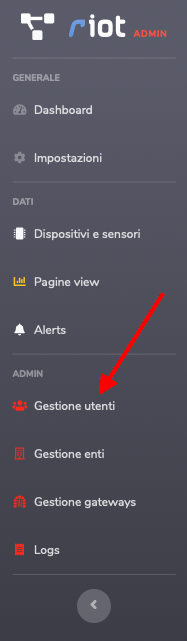
\includegraphics[scale=0.600]{res/images/admin/menuUtente.png}
		\caption{Selezione sezione utenti}
	\end{figure}
	Per entrare nella sezione di gestione utenti è necessario cliccare gestione utenti dalla sezione amministrazione del menù. 

	\subsubsection{Visualizzazione lista utenti}	
		\begin{figure}[H]
		\centering
		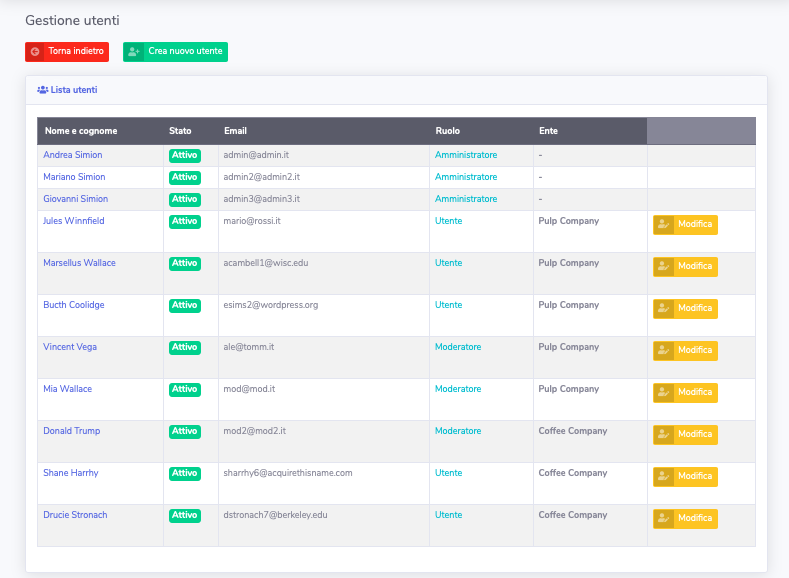
\includegraphics[scale=0.600]{res/images/admin/listaUtenti.png}
		\caption{Lista degli utenti presenti nel sistema}
	\end{figure}
	All'interno della sezione di gestione utenti è possibile vedere un elenco di tutti gli utenti del sistema con relativo id, nome e cognome, stato, email, ruolo ed eventuale ente di appartenenza. 

	\subsubsection{Visualizzazione informazioni utente}	

		\begin{figure}[H]
		\centering
		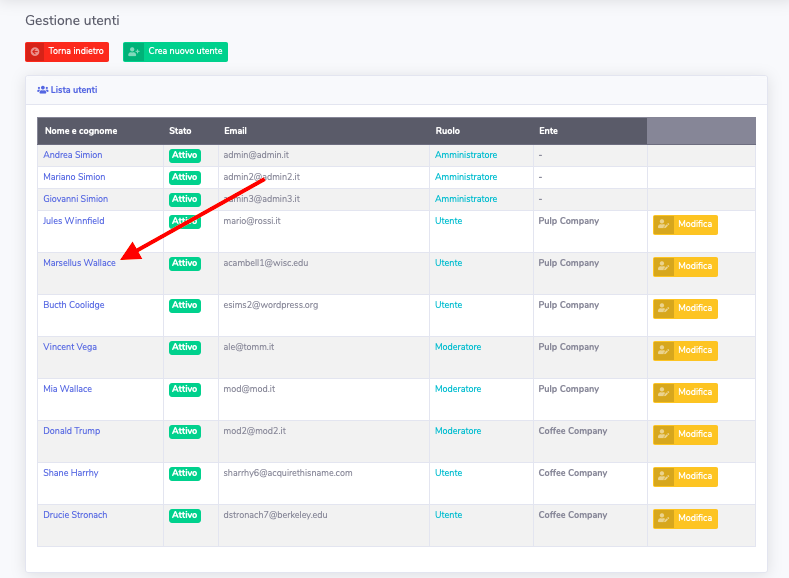
\includegraphics[scale=0.600]{res/images/admin/selDettUtente.png}
		\caption{Selezione di un utente}
	\end{figure}
	Per visualizzare le informazioni di un utente è necessario cliccare sul nome o sull'id dell'utente all'interno della lista della sezione gestione utenti.

		\begin{figure}[H]
		\centering
		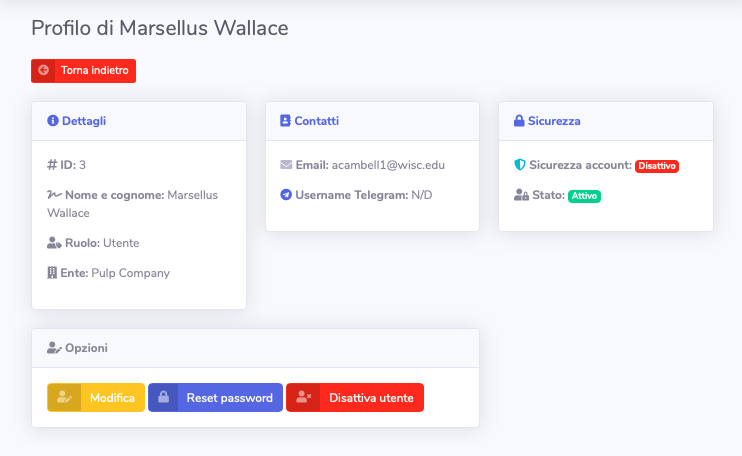
\includegraphics[scale=0.600]{res/images/admin/dettUtente.png}
		\caption{Informazioni di un utente}
	\end{figure}
	All'interno della pagina di dettaglio di un utente è possibile vedere informazioni più dettagliate dei singoli membri ed eventualmente resettare la password, disattivare l'utente o entrare nella sezione di modifica.

	\subsubsection{Creazione utente}

		\begin{figure}[H]
		\centering
		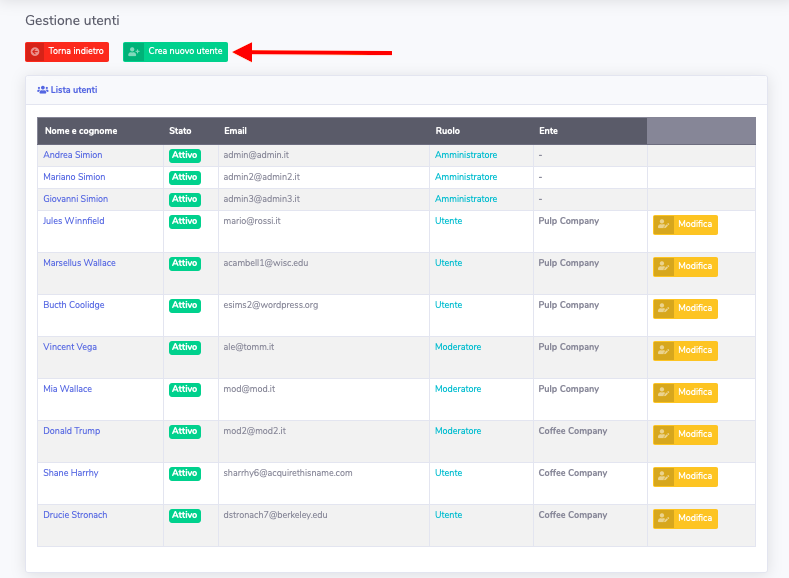
\includegraphics[scale=0.600]{res/images/admin/selCreazUtente.png}
		\caption{Creazione di un utente}
	\end{figure}
	Per creare un nuovo utente è sufficiente cliccare su "crea nuovo utente" all'interno della sezione di gestione degli utenti.

		\begin{figure}[H]
		\centering
		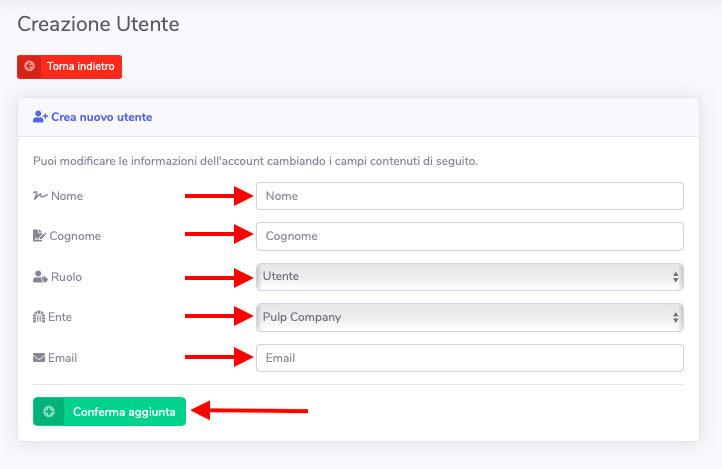
\includegraphics[scale=0.600]{res/images/admin/creazUtente.png}
		\caption{Form di creazione di un utente}
	\end{figure}
	Infine, è necessario inserire i dati richiesti nel form e cliccare su \textit{crea utente}. 
	A questo punto verrà creato un nuovo account e l'utente verrà inserito nella lista.

	\subsubsection{Modifica utente}

		\begin{figure}[H]
		\centering
		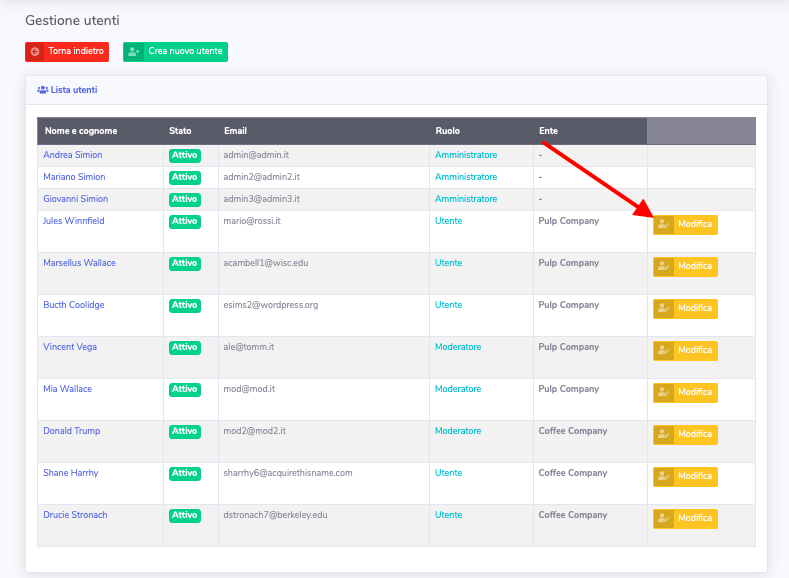
\includegraphics[scale=0.600]{res/images/admin/selModUtente.png}
		\caption{Selezione di un utente}
	\end{figure}
	Per modificare le informazioni di un utente è necessario cliccare sul bottone \textit{modifica} presente nella tabella contenente tutti gli utenti presente nella sezione gestione utenti.

		\begin{figure}[H]
		\centering
		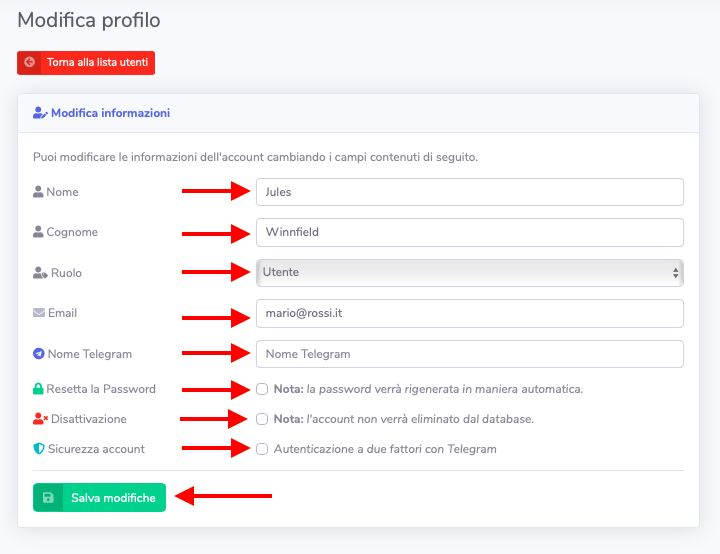
\includegraphics[scale=0.600]{res/images/admin/modUtente.png}
		\caption{Form di modifica di un utente}
	\end{figure}
	All'interno della sezione modifica è possibile modificare i dati dell'utente associato ma non solo: è possibile anche inserire il nome utente Telegram, resettare la password, disattivare l'account e attivare l'autenticazione a due fattori.
	Notare che la riassegnazione di un utente o di un moderatore a un altro ente comporta il reset di tutte le sue impostazioni sugli alert e sulle pagine view.

\newpage \subsection{12. Admin - Gestione enti}

	\begin{itemize}
		\item \href{https://www.youtube.com/watch?v=PjySMOLCtMA&list=PLPKYjnuIh1FA3b3jn_bwY_ztYzaFn2mIT&index=15}{Visualizza il video tutorial su YouTube} 
	\end{itemize}
	
	\subsubsection{Entrare nella gestione enti}

		\begin{figure}[H]
		\centering
		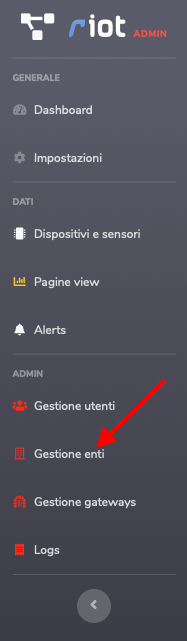
\includegraphics[scale=0.600]{res/images/admin/menuEnti.png}
		\caption{Selezione sezione enti}
	\end{figure}

		Per gestire gli enti è necessario entrare nella sezione apposita tramite il menù amministratore posto a sinistra.

	\subsubsection{Visualizzazione lista enti}

		\begin{figure}[H]
		\centering
		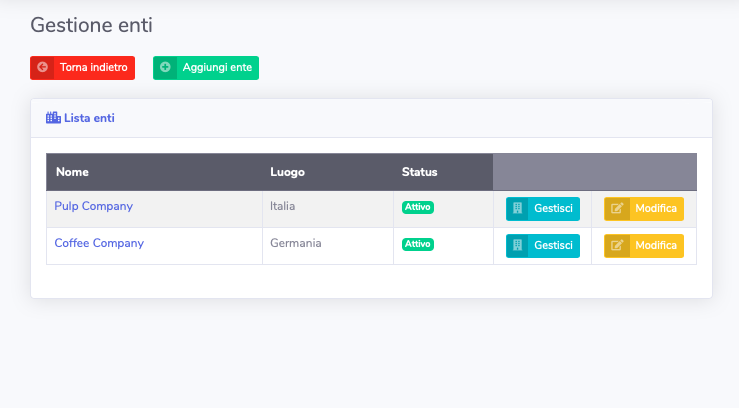
\includegraphics[scale=0.600]{res/images/admin/listaEnti.png}
		\caption{Lista degli enti presenti nel sistema}
	\end{figure}

		Per visualizzare un elenco con gli enti presenti nel sistema è necessario entrare nella sezione di gestione degli enti. All'interno di questa sezione è possibile vedere un elenco degli enti presenti nel sistema visualizzandone il nome, il luogo e lo status.			

	\subsubsection{Visualizzazione informazioni ente}

		\begin{figure}[H]
		\centering
		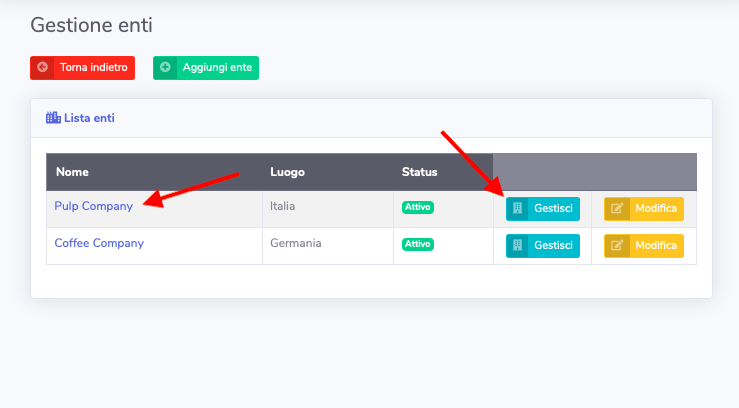
\includegraphics[scale=0.600]{res/images/admin/selDettEnte.png}
		\caption{Selezione di un ente}
	\end{figure}

		Per visualizzare le informazioni di un ente è possibile cliccare sul bottone \textit{Gestisci} presente nella lista globale degli enti all'interno della sezione di gestione degli enti. 

		\begin{figure}[H]
		\centering
		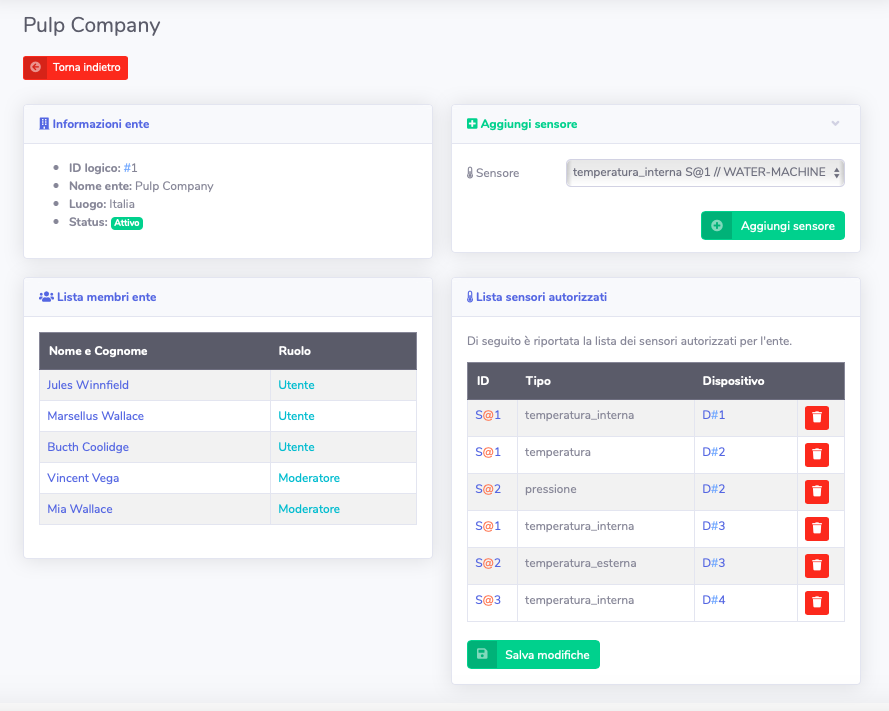
\includegraphics[scale=0.480]{res/images/admin/dettEnte.png}
		\caption{Dettagli di un ente}
	\end{figure}
	A questo punto è possibile vedere per l'ente selezionato le sue informazioni, la lista degli utenti appartenenti a quell'ente e la lista dei sensori associati.
	Alternativamente è possibile accedere ai dettagli cliccando sul nome dell'ente prescelto.

	\subsubsection{Aggiunta e rimozione sensori a un ente}

		All'interno della pagina di dettaglio di un ente, raggiungibile seguendo i passaggi elencati nelle sezioni \textbf{Entrare nella gestione enti} e \textbf{Visualizzazione informazioni ente}, è possibile aggiungere e rimuovere sensori ad un ente.

		\begin{figure}[H]
		\centering
		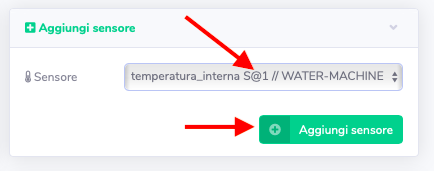
\includegraphics[scale=0.600]{res/images/admin/aggSensoreEnte.png}
		\caption{Aggiunta di un sensore ad un ente}
	\end{figure}
	Per inserire un sensore è necessario selezionare un sensore dal form presente sulla destra denominato \textit{Aggiungi sensore} e cliccare sul relativo bottone. Per rendere l'aggiunta effettiva è necessario cliccare su \textit{Salva modifiche}. 

		\begin{figure}[H]
		\centering
		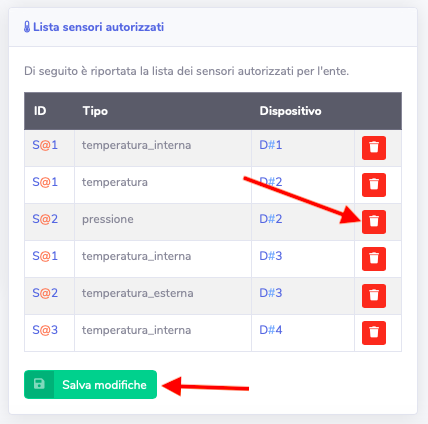
\includegraphics[scale=0.600]{res/images/admin/rimSensoreEnte.png}
		\caption{Rimozione di un sensore ad un ente}
	\end{figure}

		Per rimuovere un sensore è sufficiente premere l'icona a forma di cestino a fianco del sensore che si vuole rimuovere. Infine per rendere la rimozione effettiva è necessario cliccare su \textit{Salva modifiche}. 

	\subsubsection{Creazione ente}

		\begin{figure}[H]
		\centering
		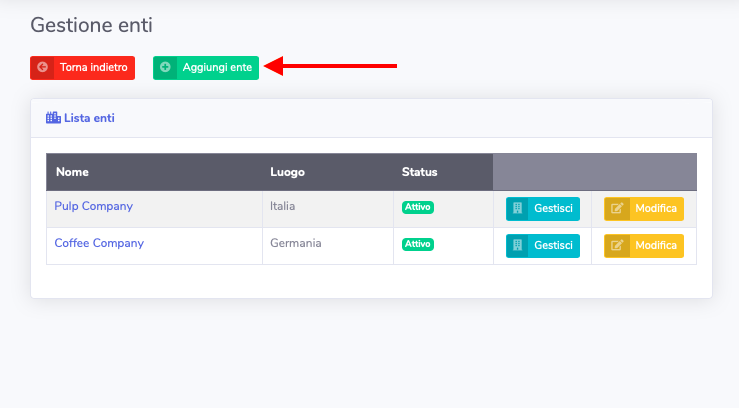
\includegraphics[scale=0.600]{res/images/admin/selCreazEnte.png}
		\caption{Creazione di un nuovo ente}
		\end{figure}

		Per aggiungere un nuovo ente è necessario cliccare su "Aggiungi ente" all'interno della sezione di gestione degli enti. 

		\begin{figure}[H]
		\centering
		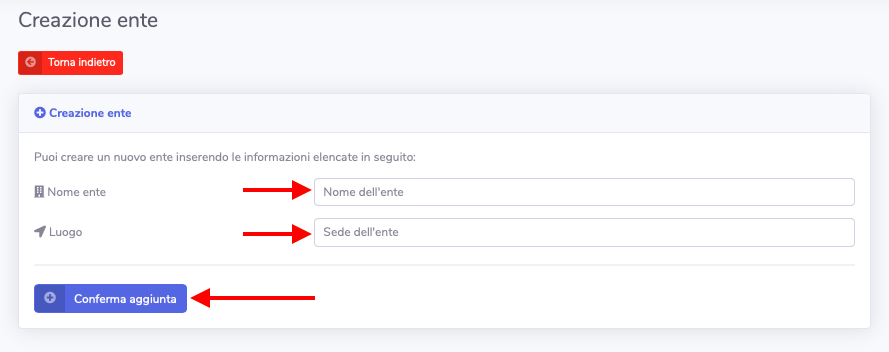
\includegraphics[scale=0.480]{res/images/admin/creazEnte.png}
		\caption{Form di creazione di un ente}
	\end{figure}

		Compilare poi il form presente nella sezione e premere "Salva".


	\subsubsection{Modifica ente}

		\begin{figure}[H]
		\centering
		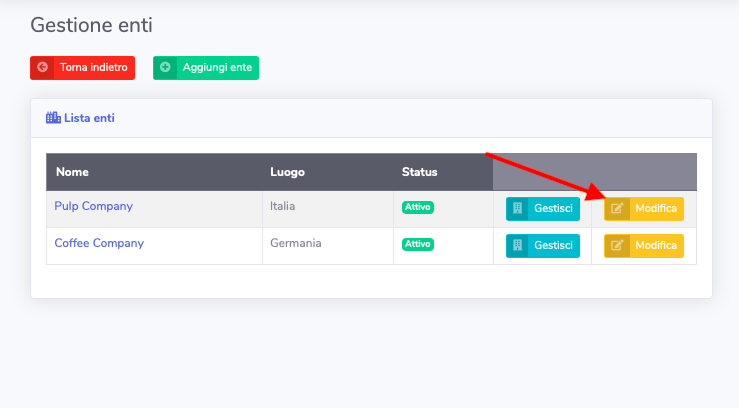
\includegraphics[scale=0.600]{res/images/admin/selModEnte.png}
		\caption{Modifica di un ente}
	\end{figure}

		Per modificare le informazioni di un ente è necessario cliccare sul bottone Modifica all'interno della sezione di gestione degli enti.

		\begin{figure}[H]
		\centering
		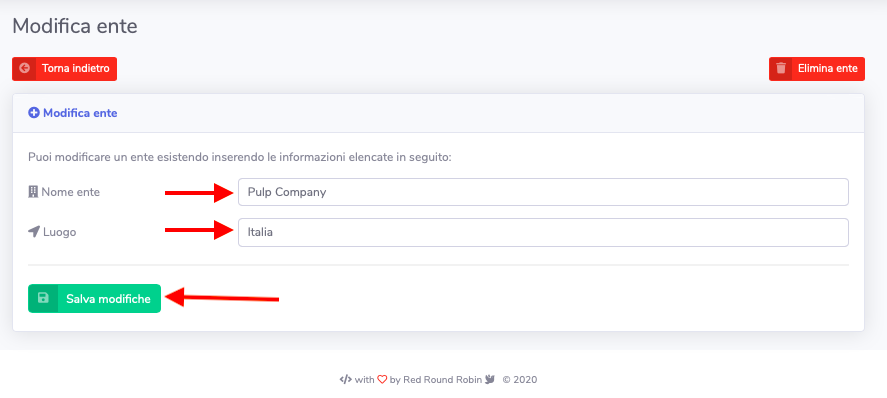
\includegraphics[scale=0.480]{res/images/admin/modEnte.png}
		\caption{Form di modifica di un ente}
	\end{figure}

		In questa sezione è possibile cambiarne il nome e il luogo. Per salvare le modifiche effettuate cliccare poi su Salva modifiche.

	\subsubsection{Eliminazione ente}	

		\begin{figure}[H]
		\centering
		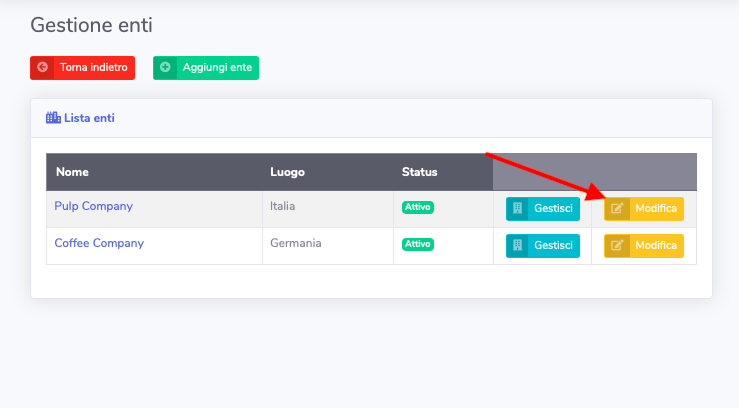
\includegraphics[scale=0.600]{res/images/admin/selModEnte.png}
		\caption{Eliminazione di un ente}
	\end{figure}


		Per eliminare un ente è necessario cliccare sul bottone Modifica all'interno della sezione di gestione degli enti.

		\begin{figure}[H]
		\centering
		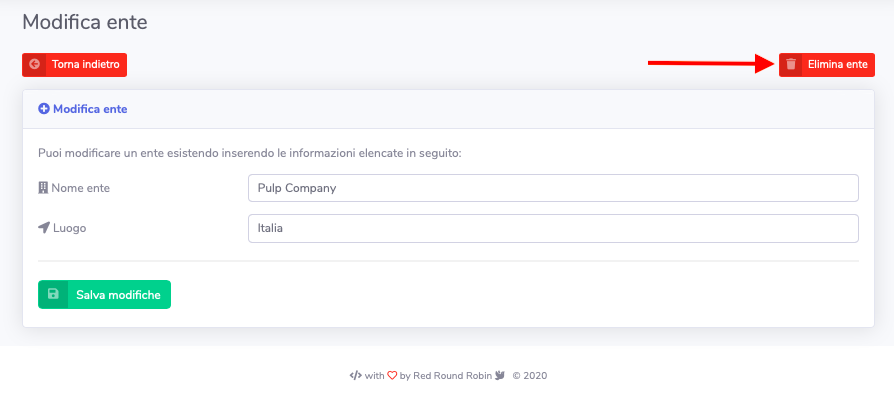
\includegraphics[scale=0.480]{res/images/admin/elimEnte.png}
		\caption{Eliminazione di un ente}
	\end{figure}


		Infine cliccare sul bottone Elimina ente posto in alto a destra.

	

\newpage \subsection{13. Admin - Gestione dispositivi}

	\begin{itemize}
		\item \href{https://www.youtube.com/watch?v=PjySMOLCtMA&list=PLPKYjnuIh1FA3b3jn_bwY_ztYzaFn2mIT&index=16}{Visualizza il video tutorial su YouTube} 
	\end{itemize}

	\subsubsection{Entrare nella gestione dispositivi}

		\begin{figure}[H]
		\centering
		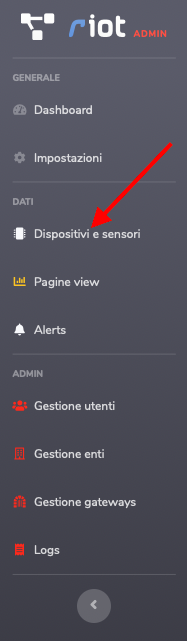
\includegraphics[scale=0.600]{res/images/admin/menuDisp.png}
		\caption{Selezione della sezione di gestione dei dispositivi}
	\end{figure}

		Per entrare entrare nella sezione di gestione dei dispositivi è sufficiente cliccare la voce Dispositivi e sensori del menù laterale.

	\subsubsection{Visualizzazione lista dispositivi}

		\begin{figure}[H]
		\centering
		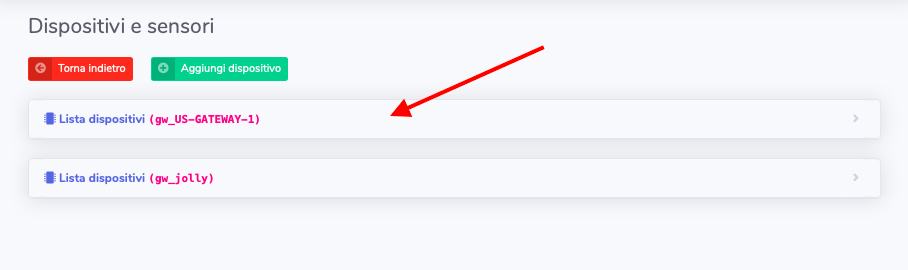
\includegraphics[scale=0.480]{res/images/admin/listaDisp.png}
		\caption{Lista dei dispositivi presenti nel sistema}
	\end{figure}

	\begin{figure}[H]
		\centering
		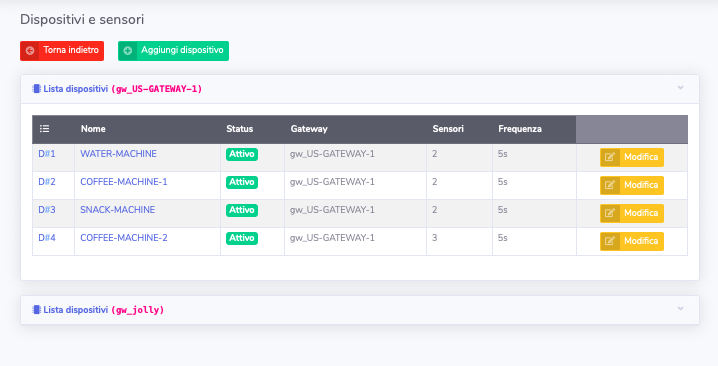
\includegraphics[scale=0.600]{res/images/admin/listaDispOpen.png}
		\caption{Lista dei dispositivi aperta}
	\end{figure}

		All'interno della sezione di gestione di dispositivi è possibile vedere per ogni gateway la lista dei dispositivi associati cliccando sul nome del gateway prescelto. 

	\subsubsection{Visualizzazione informazioni dispositivo}

		\begin{figure}[H]
		\centering
		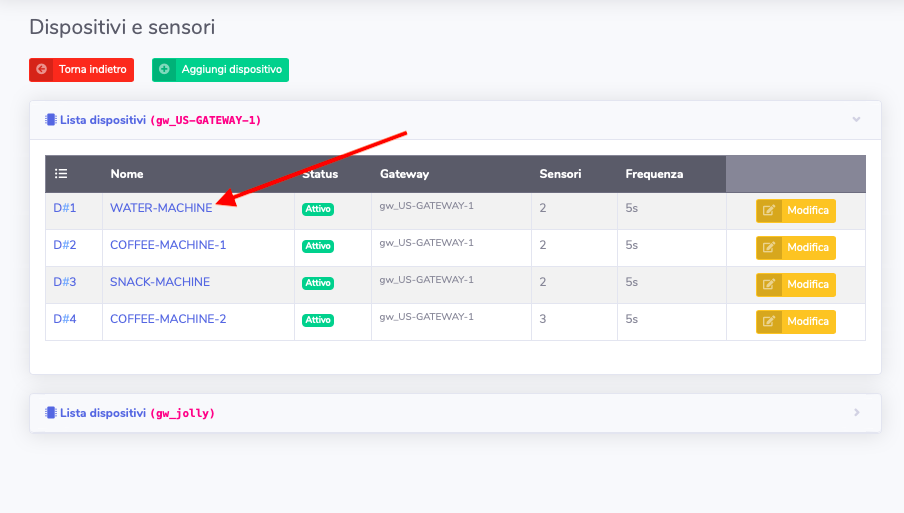
\includegraphics[scale=0.480]{res/images/admin/selDetDisp.png}
		\caption{Selezione di un dispositivo}
	\end{figure}


		\begin{figure}[H]
		\centering
		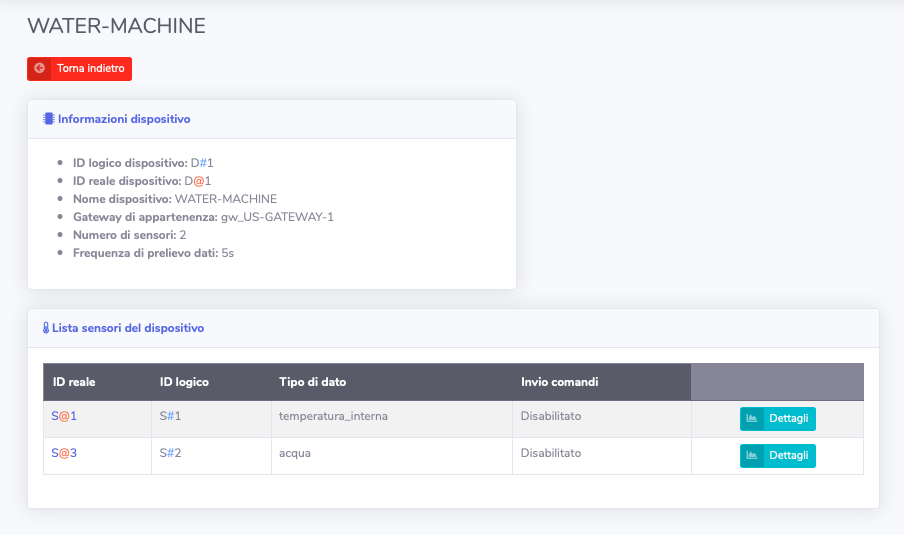
\includegraphics[scale=0.480]{res/images/admin/dettDisp.png}
		\caption{Dettagli di un dispositivo}
	\end{figure}


		Per visualizzare le informazioni di un dispositivo, cliccare sul nome o l'id del dispositivo prescelto all'interno della lista di dispositivi visualizzabile nella sezione di gestione dei dispositivi.

	\subsubsection{Visualizzazione dettaglio sensore}

		\begin{figure}[H]
		\centering
		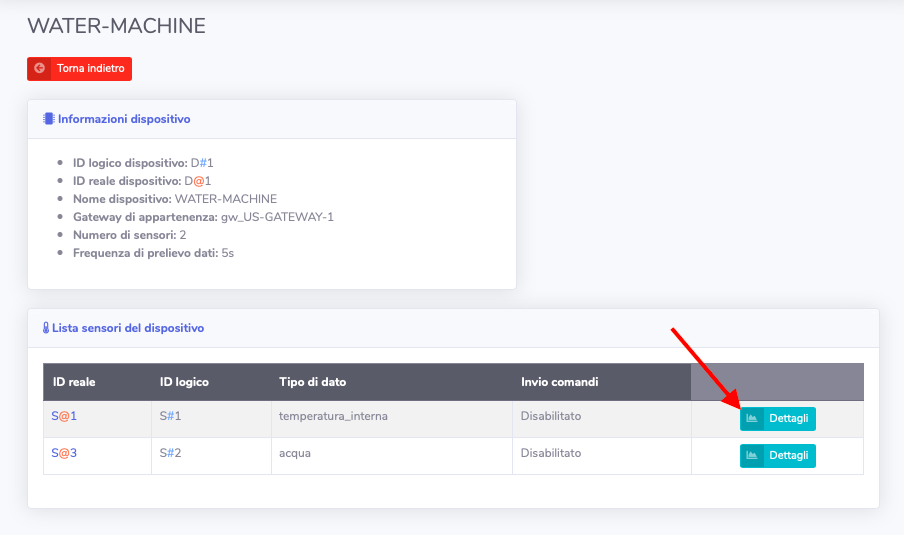
\includegraphics[scale=0.480]{res/images/admin/selDettSens.png}
		\caption{Selezione di un sensore}
	\end{figure}


		Per visualizzare le informazioni di un sensore è necessario cliccare sul bottone Dettagli presente all'interno della lista dei sensori di un determinato dispositivo (Visualizzabile seguendo la sezione \textbf{Visualizzazione informazioni dispositivo}).

		\begin{figure}[H]
		\centering
		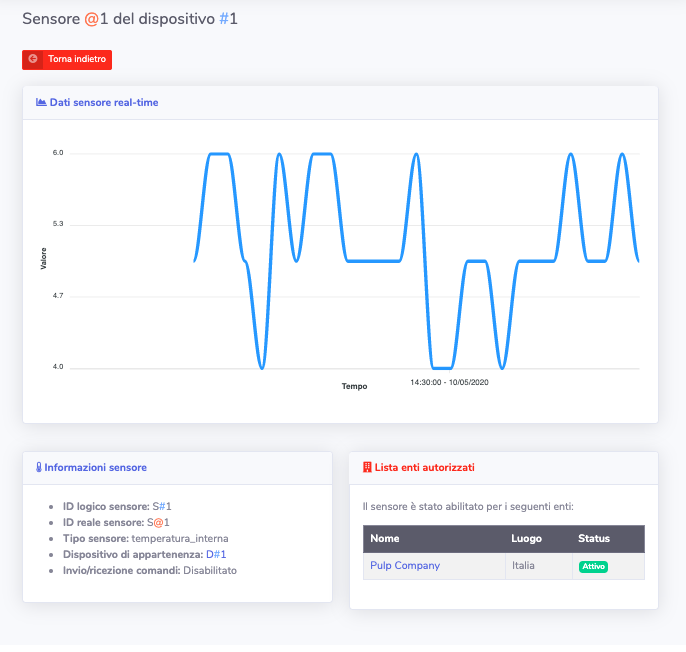
\includegraphics[scale=0.600]{res/images/admin/dettSensore.png}
		\caption{Dettagli di un sensore}
	\end{figure}


		All'interno della pagina è possibile visualizzare le informazioni di un dispositivo, il grafico con i suoi valori di output e la lista degli enti a cui è stato assegnato.

	\subsubsection{Creazione dispositivo}

		\begin{figure}[H]
		\centering
		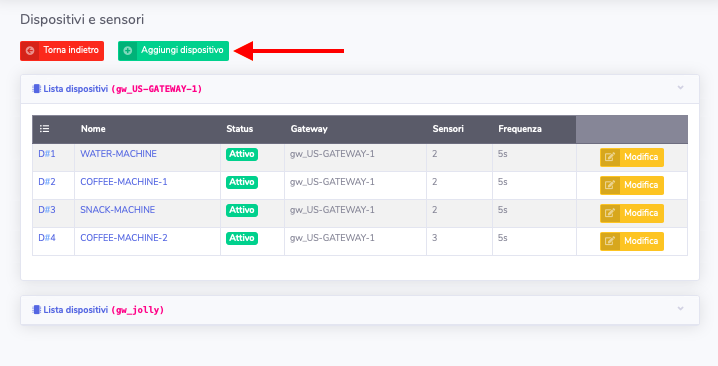
\includegraphics[scale=0.600]{res/images/admin/selCreazDisp.png}
		\caption{Creazione di un dispositivo}
	\end{figure}


		All'interno della sezione di gestione dei dispositivi è possibile creare un nuovo dispositivo cliccando sul bottone Aggiungi dispositivo. 

		\begin{figure}[H]
		\centering
		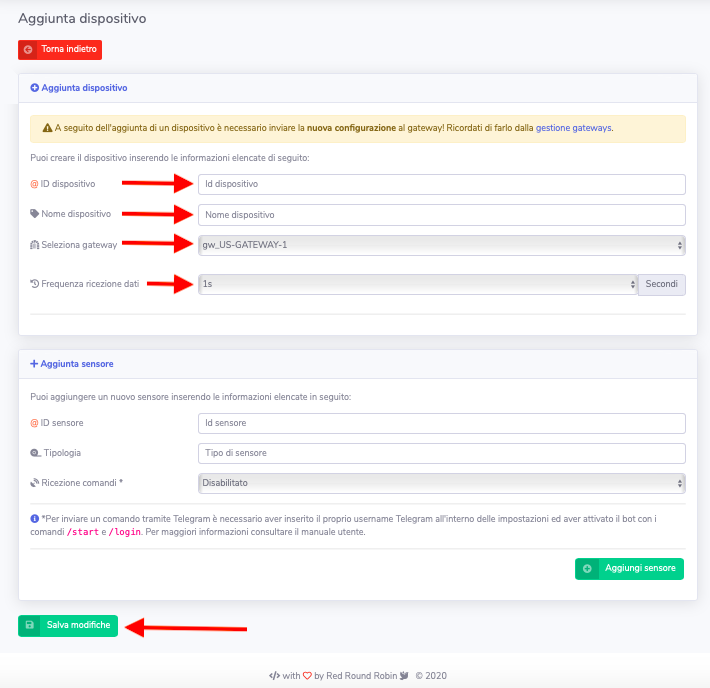
\includegraphics[scale=0.600]{res/images/admin/creazDisp.png}
		\caption{Form di creazione di un dispositivo}
	\end{figure}

		A questo punto è possibile creare un dispositivo inserendo il suo id reale, il nome, il gateway di appartenenza e la frequenza di ricezione dei dati. 

		\begin{figure}[H]
		\centering
		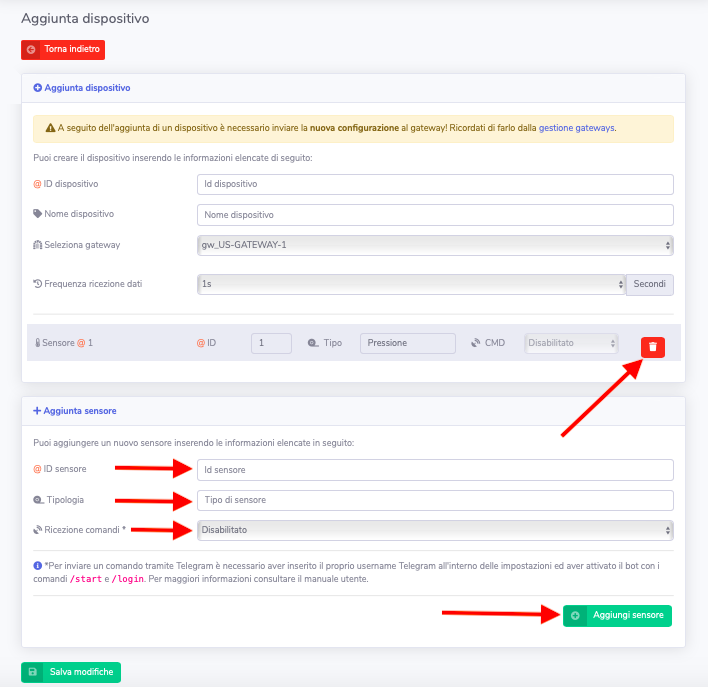
\includegraphics[scale=0.600]{res/images/admin/aggRimSens.png}
		\caption{Form di aggiunta e rimozione di un sensore}
	\end{figure}

		Per inserire inserire uno o più sensori è necessario compilare il form sottostante inserendo l'id reale del sensore, la sua tipologia e scegliendo se il sensore può o meno ricevere dei comandi. Infine cliccare su Aggiungi sensore.
		Per salvare i dati inseriti nel nuovo dispositivo cliccare su Salva modifiche.
		Notare che per propagare le modifiche anche sui gateway, sarà necessario inviare la nuova configurazione tramite l'apposita pagina di \textit{Gestione Gateway}.

	\subsubsection{Modifica dispositivo}

		\begin{figure}[H]
		\centering
		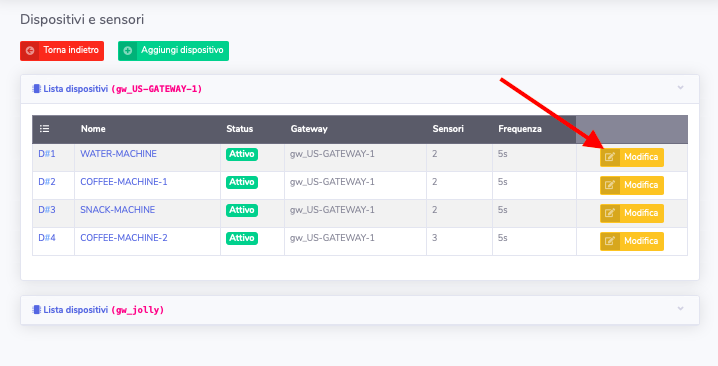
\includegraphics[scale=0.600]{res/images/admin/selModDisp.png}
		\caption{Modifica di un dispositivo}
	\end{figure}

		Per modificare un dispositivo è necessario entrare nella sezione di gestione dei dispositivi e cliccare sul bottone Modifica associato al dispositivo prescelto.

		\begin{figure}[H]
		\centering
		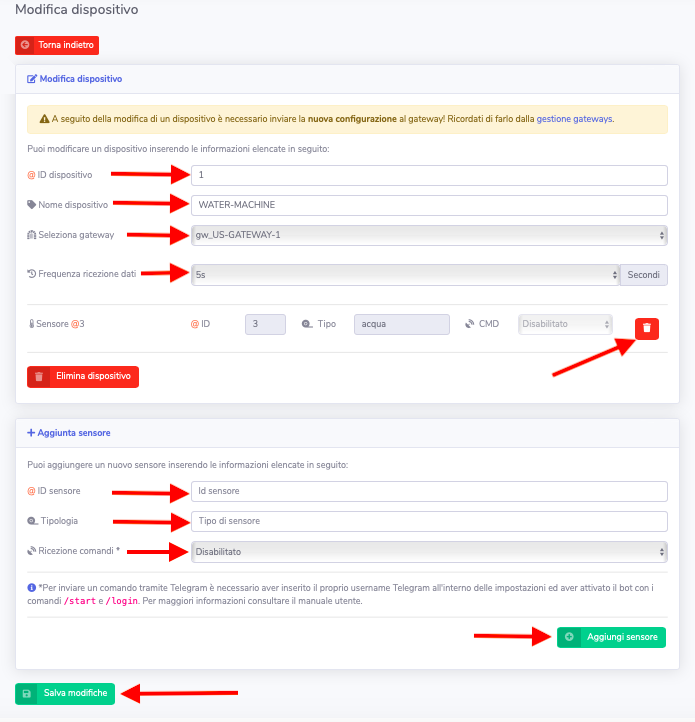
\includegraphics[scale=0.600]{res/images/admin/modDispositivo.png}
		\caption{Form di modifica di un dispositivo}
	\end{figure}

		A questo punto è necessario modificare i dati ed infine cliccare su Salva modifiche. 
		Notare che per propagare le modifiche anche sui gateway, sarà necessario inviare la nuova configurazione tramite l'apposita pagina di \textit{Gestione Gateway}.

	\subsubsection{Eliminazione dispositivo}	

		\begin{figure}[H]
		\centering
		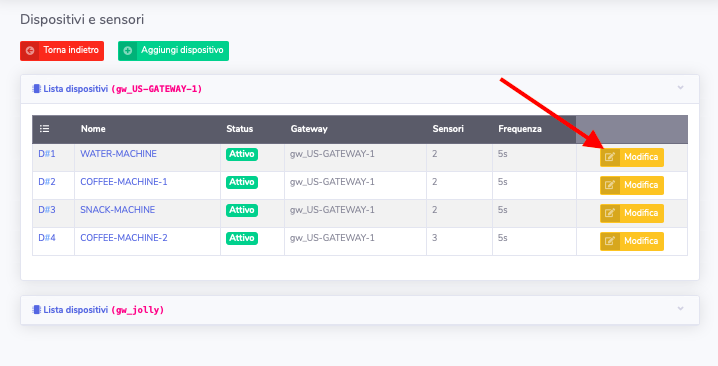
\includegraphics[scale=0.600]{res/images/admin/selModDisp.png}
		\caption{Eliminazione di un dispositivo}
	\end{figure}


		Per eliminare un dispositivo è necessario entrare nella sezione di gestione dei dispositivi e cliccare sul bottone Modifica associato al dispositivo prescelto. 

		\begin{figure}[H]
		\centering
		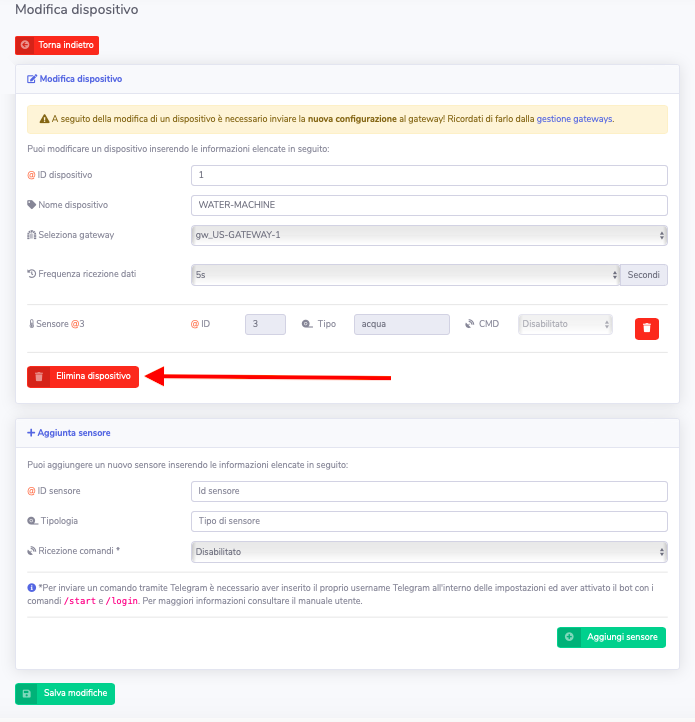
\includegraphics[scale=0.600]{res/images/admin/elimDisp.png}
		\caption{Eliminazione di un dispositivo}
	\end{figure}

		All'interno di questa pagina è poi sufficiente cliccare sul bottone Elimina dispositivo posto sotto al form di inserimento dei dati del dispositivo.
		Notare che per propagare le modifiche anche sui gateway, sarà necessario inviare la nuova configurazione tramite l'apposita pagina di \textit{Gestione Gateway}.

\newpage \subsection{14. Admin - Gestione gateway}
	
	\begin{itemize}
		\item \href{https://www.youtube.com/watch?v=PjySMOLCtMA&list=PLPKYjnuIh1FA3b3jn_bwY_ztYzaFn2mIT&index=17}{Visualizza il video tutorial su YouTube} 
	\end{itemize}

	\subsubsection{Entrare nella gestione gateway}

		\begin{figure}[H]
		\centering
		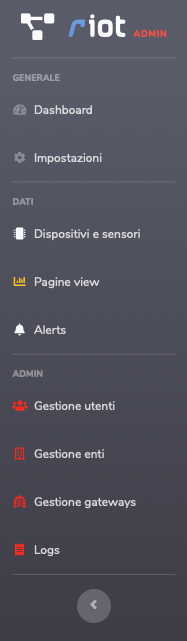
\includegraphics[scale=0.600]{res/images/admin/menuGateway.png}
		\caption{}
	\end{figure}

		Per entrare entrare nella sezione di gestione dei gateway è sufficiente cliccare la voce Gestione gateways del menù laterale.

	\subsubsection{Visualizzazione lista gateway}

		\begin{figure}[H]
		\centering
		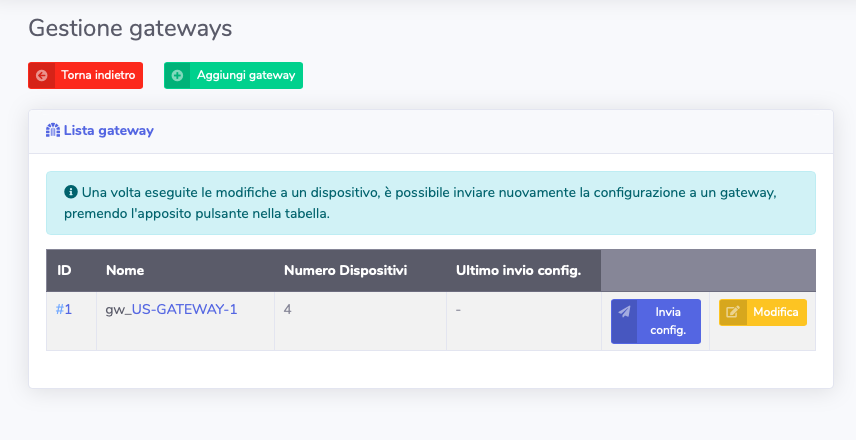
\includegraphics[scale=0.500]{res/images/admin/listaGateway.png}
		\caption{Lista dei gateway presenti nel sistema}
	\end{figure}

		All'interno della sezione di gestione gateway è possibile visualizzare la lista dei gateway disponibili nel sistema e le relative informazioni.

	\subsubsection{Visualizzazione informazioni gateway}

		\begin{figure}[H]
		\centering
		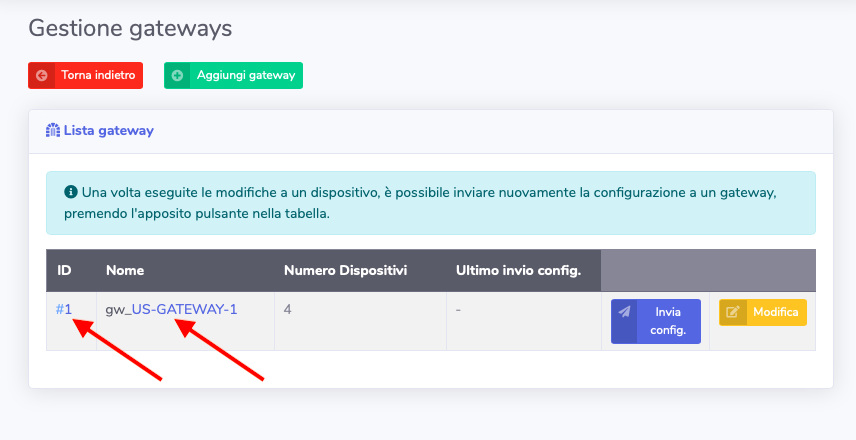
\includegraphics[scale=0.500]{res/images/admin/selDettGateway.png}
		\caption{Selezione di un gateway}
	\end{figure}


		Le informazioni più dettagliate dei gateway sono disponibili a partire dalla sezione Gestione gateways in cui è presente la lista dei gateways presenti nel sistema.

		\begin{figure}[H]
		\centering
		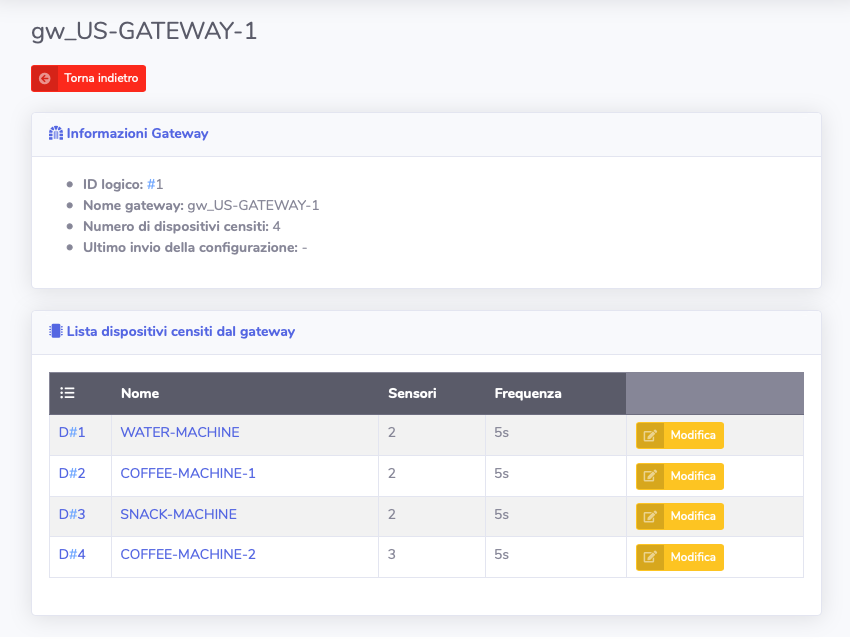
\includegraphics[scale=0.500]{res/images/admin/dettGateway.png}
		\caption{Dettagli di un gateway}
	\end{figure}

		Da questa sezione è possibile cliccare sul nome o l'ID del gateway prescelto e quindi visualizzarne le informazioni e lista dei dispositivi associati.

	\subsubsection{Creazione gateway}

		\begin{figure}[H]
		\centering
		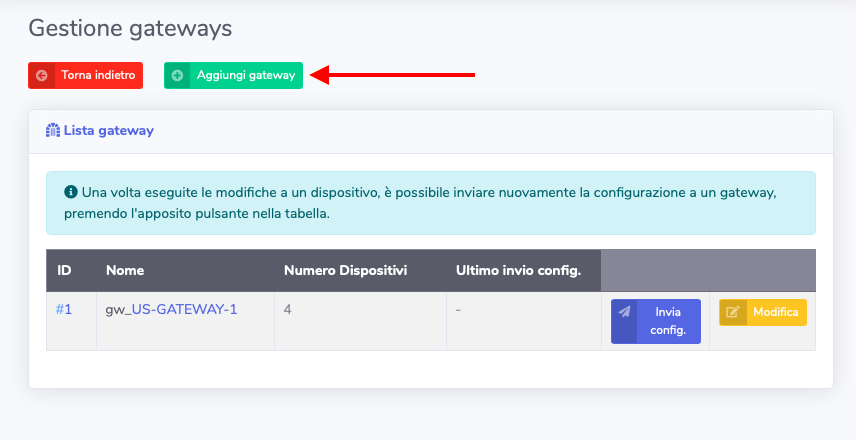
\includegraphics[scale=0.500]{res/images/admin/selCreazGateway.png}
		\caption{Creazione di un gateway}
	\end{figure}


		Per creare un nuovo gateway è necessario cliccare su Aggiungi gateway a partire dalla lista dei gateway disponibili.

		\begin{figure}[H]
		\centering
		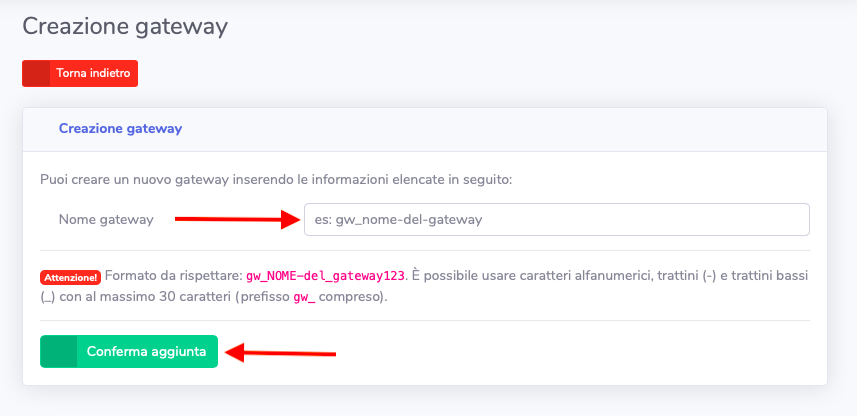
\includegraphics[scale=0.500]{res/images/admin/creazGateway.png}
		\caption{Form di creazione di un gateway}
	\end{figure}


		Nella nuova pagina poi compilare il form presente e cliccare su Conferma aggiunta. 

	\subsubsection{Modifica gateway}

		\begin{figure}[H]
		\centering
		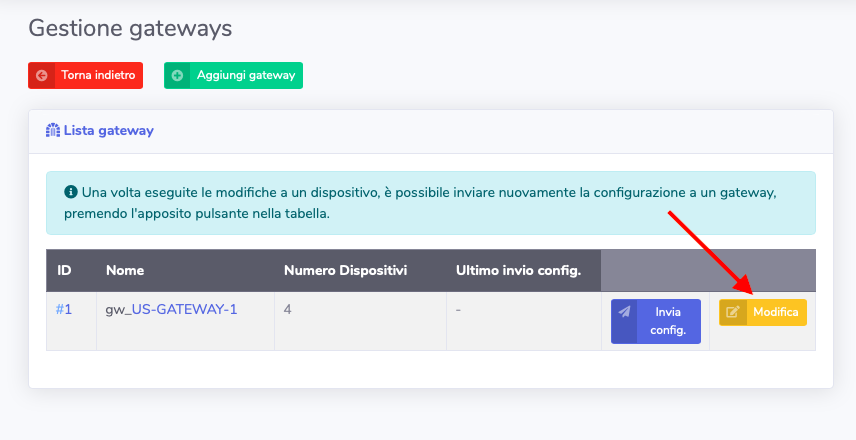
\includegraphics[scale=0.500]{res/images/admin/selModGateway.png}
		\caption{Modifica di un gateway}
	\end{figure}

		Per modificare le informazioni di un gateway preesistente è necessario cliccare sul bottone Modifica presente nella lista dei gateway presenti nel sistema e successivamente modificarne le informazioni.

		\begin{figure}[H]
		\centering
		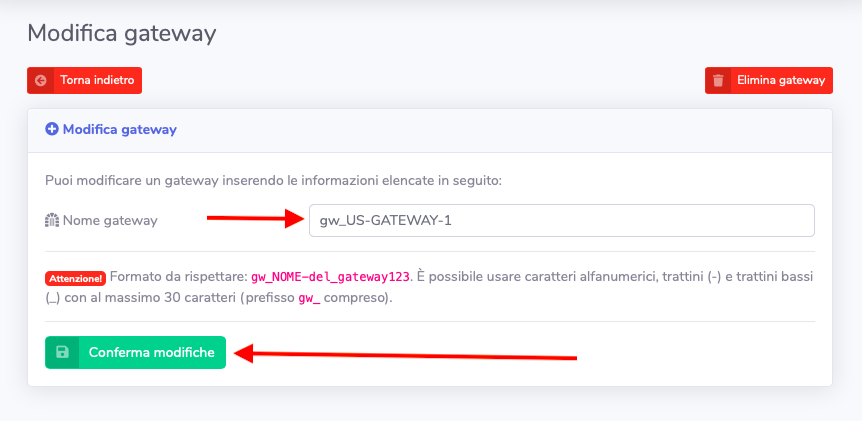
\includegraphics[scale=0.500]{res/images/admin/modGateway.png}
		\caption{Form di modifica di un gateway}
	\end{figure}

		Infine è necessario cliccare su Conferma modifiche per renderle permanenti.

	\subsubsection{Eliminazione gateway}

		\begin{figure}[H]
		\centering
		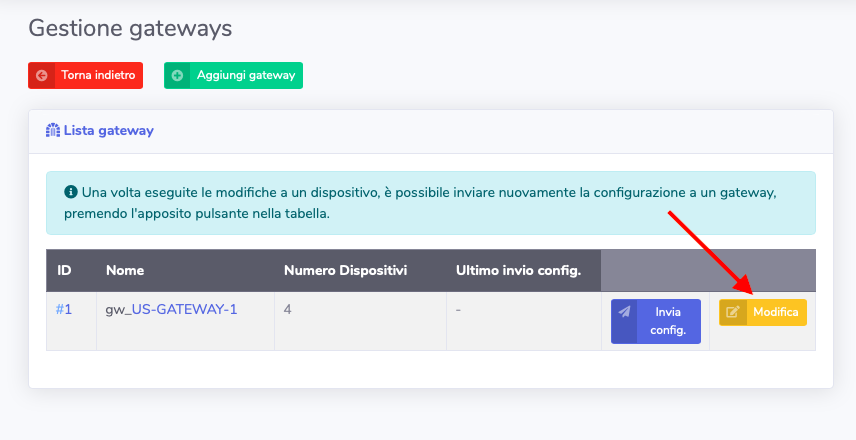
\includegraphics[scale=0.500]{res/images/admin/selModGateway.png}
		\caption{Eliminazione di un gateway}
	\end{figure}

		\begin{figure}[H]
		\centering
		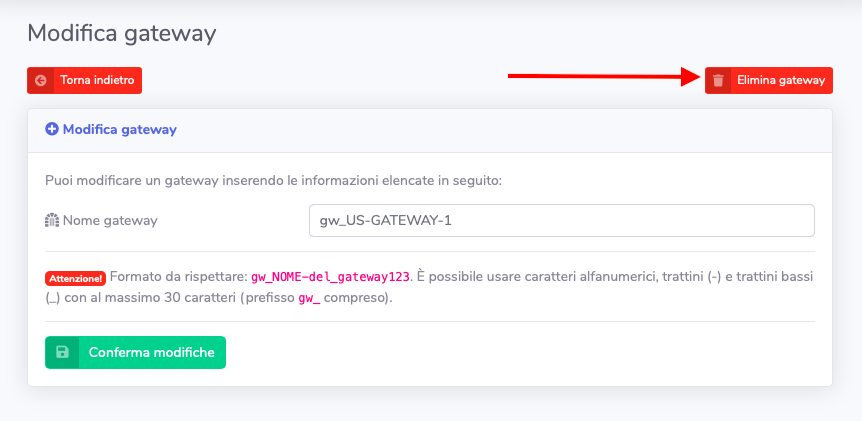
\includegraphics[scale=0.500]{res/images/admin/elimGateway.png}
		\caption{Eliminazione di un gateway}
	\end{figure}


		Per eliminare un gateway preesistente è necessario cliccare sul bottone Modifica presente nella lista dei gateway presenti nel sistema e successivamente premere sul bottone Elimina.

	\subsubsection{Invio configurazione}

		Per inviare una nuova configurazione di un gateway, entrare nella sezione di gestione dei gateways.

		\begin{figure}[H]
		\centering
		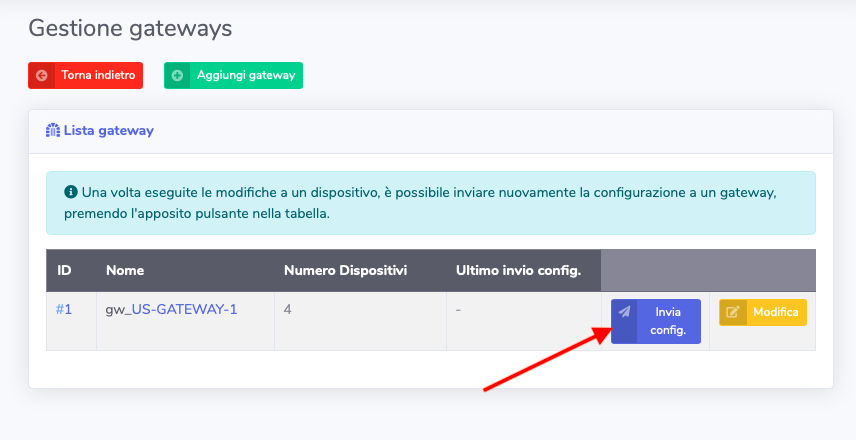
\includegraphics[scale=0.500]{res/images/admin/inviaConfig.png}
		\caption{Invio di una configurazione}
	\end{figure}

		Da qui è necessario cliccare sul bottone \textit{Invia config} associato al gateway di cui si vuole inviare la configurazione.


\newpage \subsection{15. Admin - Logs e Alerts}

	\begin{itemize}
		\item \href{https://www.youtube.com/watch?v=PjySMOLCtMA&list=PLPKYjnuIh1FA3b3jn_bwY_ztYzaFn2mIT&index=18}{Visualizza il video tutorial su YouTube} 
	\end{itemize}
	
	\subsubsection{Visualizzazione logs}

	\begin{figure}[H]
		\centering
		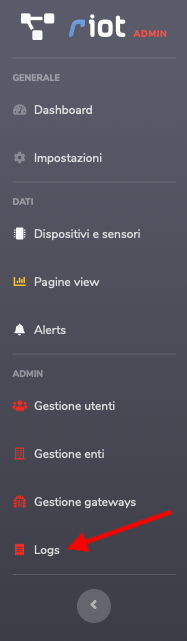
\includegraphics[scale=0.600]{res/images/admin/menuLogs.png}
		\caption{Selezione della voce logs dal menù}
	\end{figure}

		Per visualizzare i logs degli utenti del sistema è necassario entrare nella sezione Logs del menù di amministrazione.

	\begin{figure}[H]
		\centering
		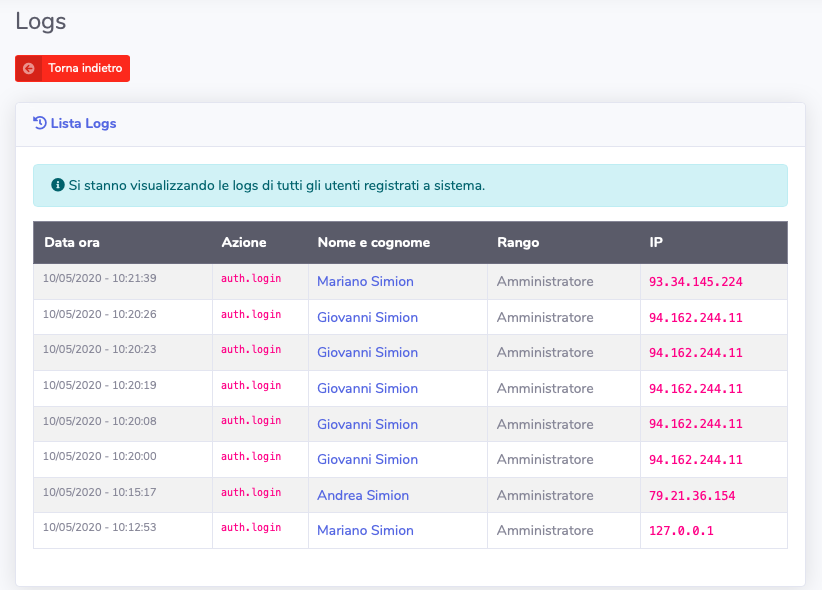
\includegraphics[scale=0.600]{res/images/admin/logs.png}
		\caption{Logs del sistema}
	\end{figure}

	In questa sezione è possibile vedere le azioni compiute da tutti gli utenti, visualizzandone la data e l'ore, il nome e cognome, l'azione, il rango dell'utente e l'indirizzo IP.

	\subsubsection{Visualizzazione alerts}

	\begin{figure}[H]
		\centering
		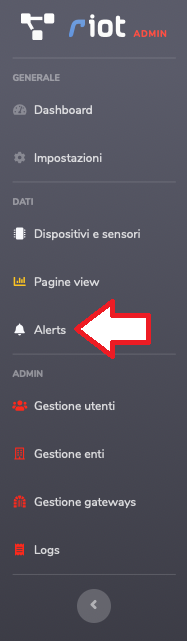
\includegraphics[scale=0.600]{res/images/admin/menuAlerts.png}
		\caption{Selezione della voce logs dal menù}
	\end{figure}

		Per visualizzare gli alert attivi nel sistema è necassario entrare nella sezione Alerts del menù di amministrazione.

	\begin{figure}[H]
		\centering
		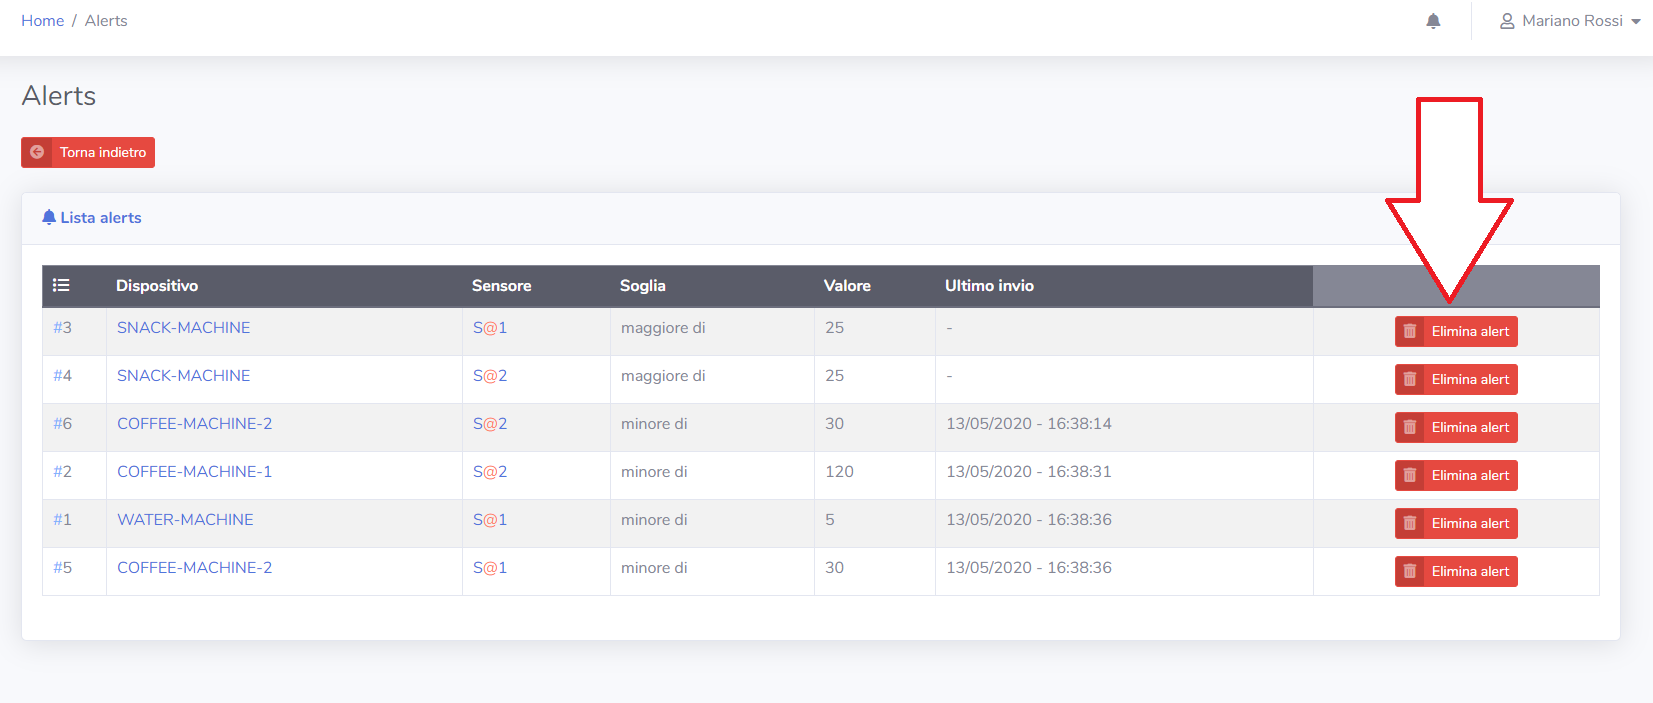
\includegraphics[scale=0.350]{res/images/admin/elimAlert.png}
		\caption{Logs del sistema}
	\end{figure}

	In questa sezione è possibile vedere gli alert attivati da parte dei moderatori degli enti, con le relative soglie impostate. Cliccando su \textbf{Elimina Alert} sarà possibile rimuovere questo alert dal sistema e tutte le impostazioni relative alle notifiche di quell'alert specifico verranno rimosse per tutti gli utenti. L'operazione non è reversibile da database. 